% begin module improper-integral-comparison
\begin{frame}
\frametitle{A Comparison Test for Improper Integrals}
Sometimes it's impossible to find the exact value of an integral, but we still want to know if it's convergent or divergent.  For such cases, we can sometimes use the following theorem.
\begin{theorem}[Comparison Theorem]
Suppose $f$ and $g$ are continuous and $f(x) \geq g(x) \geq 0$ for $x \geq a$.
\begin{enumerate}
\item  \alertNoH{2}{If $\int_a^\infty f(x) \diff x$ is convergent}, then \alertNoH{3}{$\int_a^\infty g(x)\diff x$ is convergent}.
\item \alertNoH{4}{If $\int_a^\infty g(x) \diff x$ is divergent}, \alertNoH{5}{then $\int_a^\infty f(x)\diff x$ is divergent.}
\end{enumerate}
\end{theorem}
\begin{columns}[c]
\column{.4\textwidth}
%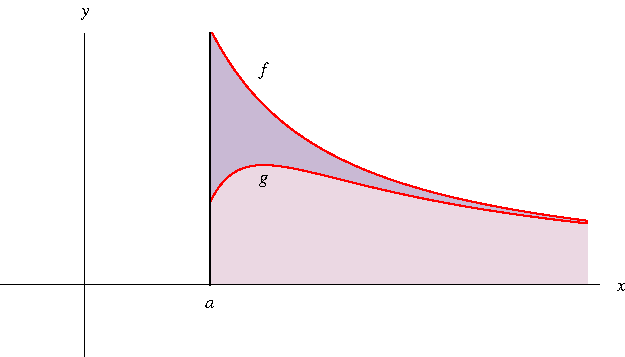
\includegraphics[height=3cm]{improper-integrals/pictures/08-08-comptest.pdf}%
\psset{xunit=0.5cm, yunit=0.5cm}
\begin{pspicture}(-0.5, -0.5)(8.6,5.4)
\psframe*[linecolor=white](-0.5,-0.5)(8.6,5.4)
\tiny

\pscustom*[linecolor=blue]{
%Function formula: \frac{4}{(x-1/2)^{1/2}}
\psplot[linecolor=\fcColorGraph, plotpoints=1000]{1.100000} {8.5} {4.0000000 -0.5000000 x add 0.5000000 exp div }\psline(8.5, 0)(1.100000, 0)}


\pscustom*[linecolor=cyan]{
%Function formula: \frac{8 x-4}{x^{2}+2}
\psplot[linecolor=\fcColorGraph, plotpoints=1000]{1.100000} {8.5} {-4.0000000 x 8.0000000 mul add 2.0000000 x 2.0000000 exp add div } 
\psline(8.5, 0)(1.100000, 0)
}

\uncover<handout:0|3,4>{
\pscustom*[linecolor=red]{
%Function formula: \frac{8 x-4}{x^{2}+2}
\psplot[linecolor=\fcColorGraph, plotpoints=1000]{1.100000} {8.5} {-4.0000000 x 8.0000000 mul add 2.0000000 x 2.0000000 exp add div } 
\psline(8.5, 0)(1.100000, 0)
}
}

\uncover<handout:0|2,5>{
\pscustom*[linecolor=red]{
%Function formula: \frac{4}{(x-1/2)^{1/2}}
\psplot[linecolor=\fcColorGraph, plotpoints=1000]{1.100000} {8.5} {4.0000000 -0.5000000 x add 0.5000000 exp div }\psline(8.5, 0)(1.100000, 0)}
}


%Function formula: \frac{4}{(x-1/2)^{1/2}}
\psplot[linecolor=\fcColorGraph, plotpoints=1000]{1.100000} {8.500000} {4.0000000 -0.5000000 x add 0.5000000 exp div }
%Function formula: \frac{8 x-4}{x^{2}+2}
\psplot[linecolor=\fcColorGraph, plotpoints=1000] {1.100000} {8.5000000}{-4.0000000 x 8.0000000 mul add 2.0000000 x 2.0000000 exp add div }


\fcAxesStandardNoFrame{-0.500000}{-0.5}{8.6}{5.3}
\uncover<handout:0|2,3>{\rput(4.2,1){Area$<\infty$}}
\uncover<handout:0|4,5>{\rput(4.2,1){Area$=\infty$}}

\rput(2,4){$f$}
\rput(2,1.4){$g$}
\psline(1.1, 0)(1.1, 5.163977795)
\end{pspicture}

\column{.6\textwidth}
\uncover<7->{%
A similar theorem holds for Type II improper integrals.
}%
\end{columns}
\end{frame}
% end module improper-integral-comparison
